\part{Modélisation du théâtre d’Orange}

	\chapter*{Introduction}
	\addcontentsline{toc}{chapter}{Introduction}
	
			 Le théâtre antique d'Orange situé dans le Vaucluse est le théâtre romain le mieux conservé d'Europe et un des trois seul au monde a avoir conservé son mur de scène. Il est adossé à la colline Saint-Eutrope sur laquelle sa \gls{cavea} repose partiellement.
			 
			 En 45 avant notre ère, suite à la victoire de César sur la Gaulle, de larges vagues de colonisation amenèrent des soldats vétérans à s'installer dans la province de Gaule transalpine qu'August réorganise par la suite en province de Narbonnaise. L'architecture urbaine est alors régie par les écrits de \cite{vitruve} et de nombreux théâtres sont construit comme celui d'Arles en 20 avant notre ère. La construction du théâtre de la "Colonia Firmus Iulius Secundanorum Aurosio" (l'ancienne ville d'Orange) fut démarré par les vétérans de la II\up{e} légion gallique de César vers 10 avant notre ère et dura près quelques dizaines d'années. \citep{PouvoirDuTheatre}
			 
			 Lorsque le théâtre fut abandonné comme édifice de spectacle, il ne fut pas détruit. Les princes d'Orange y firent installer un poste avancé de leur château et l’ensemble de l’édifice fut investi par des habitations utilisant le mur de scène comme rempart de protection. Au XVII\up{e} siècle le roi Louis XIV qualifiait en ces mots son impressionnant mur de scène de 103m de large par 37m de haut comme : « La plus belle muraille de mon royaume » et quelques écrits tentèrent d'imaginer les démonstrations qui pouvaient se tenir dans ce lieu de spectacle. 
			 
			 Ce n'est pourtant qu'au XIX\up{e} siècle que débuta un vaste chantier de déblaiement de l'enceinte dans le but de restituer au bâtiment son rôle premier. Avec ce projet apparurent les premières images d'archive du théâtre. En charge du chantier, Augustin Caristie fait paraitre en 1846, \textit{"Monuments antiques à Orange, arc triomphe et théâtre"} oeuvre de référence qui recense l'état des vestiges avant et après la destruction des maisons. Ces textes et dessins bien que, comme le stipule l'auteur, parfois hypothétiques sont par la suite complétés par d'autres architectes comme Pierre-Honoré Daumet qui réalisa en 1873 le relevé des élévations du monument. Les premières représentations théâtrales modernes purent alors avoir lieu. \`{A} la fin du siècle l'architecte Jean-Camille Formigé fut chargé de restaurer la cavea selon les indications de Caristie et en s'inspirant du modele de Vitruve. Son fils Jules Formigé poursuivit son travail et mis à jour de nombreux éléments de décors notamment en creusant au niveau de l'\gls{hyposcaenium}. Depuis les années 20 jusqu'aux années 80 de nombreuse reconstructions ont été effectués avec une rigueur archéologique contestable dans le but principalement d'habiller le lieu plus que pour le restituer. En 1981 le théâtre entre au patrimoine mondiale de l'UNESCO et quelques années plus tard d'autres constructions modernes tels que la couverture métallique de la scène viennent s'ajouter, détériorant au passage une partie de la maçonnerie antique. Certains projets ont pu être stoppés avant que des dégâts irréparables ne soient créer comme la créations d'ascenseurs dans le mur de scène. Malgré tout, ces travaux ont souvent été entrepris sans le moindre regard archéologique et de nombreuses données ont été perdues \citep{carteArcheo}.
			 
			 Depuis la fin du XX\up{e} siècle l'\gls{iraa} a relancé une étude approfondie du bâtiment et de sa décoration avec une approche archéologique rigoureuse. C'est dans cette démarche que cette thèse s'interface avec pour objectif la modélisation numérique du théâtre. Dans cette première partie nous allons donc présenter l'agencement architectural du bâtiment sans entrer dans les détails de sa décoration. Nous détaillerons ensuite les méthodes de modélisation graphique utilisées et finirons par exposer les nouveaux éléments archéologiques découlant de ce travail.
			 
		
\begin{figureth}
	\begin{subfigureth}{0.49\textwidth}
		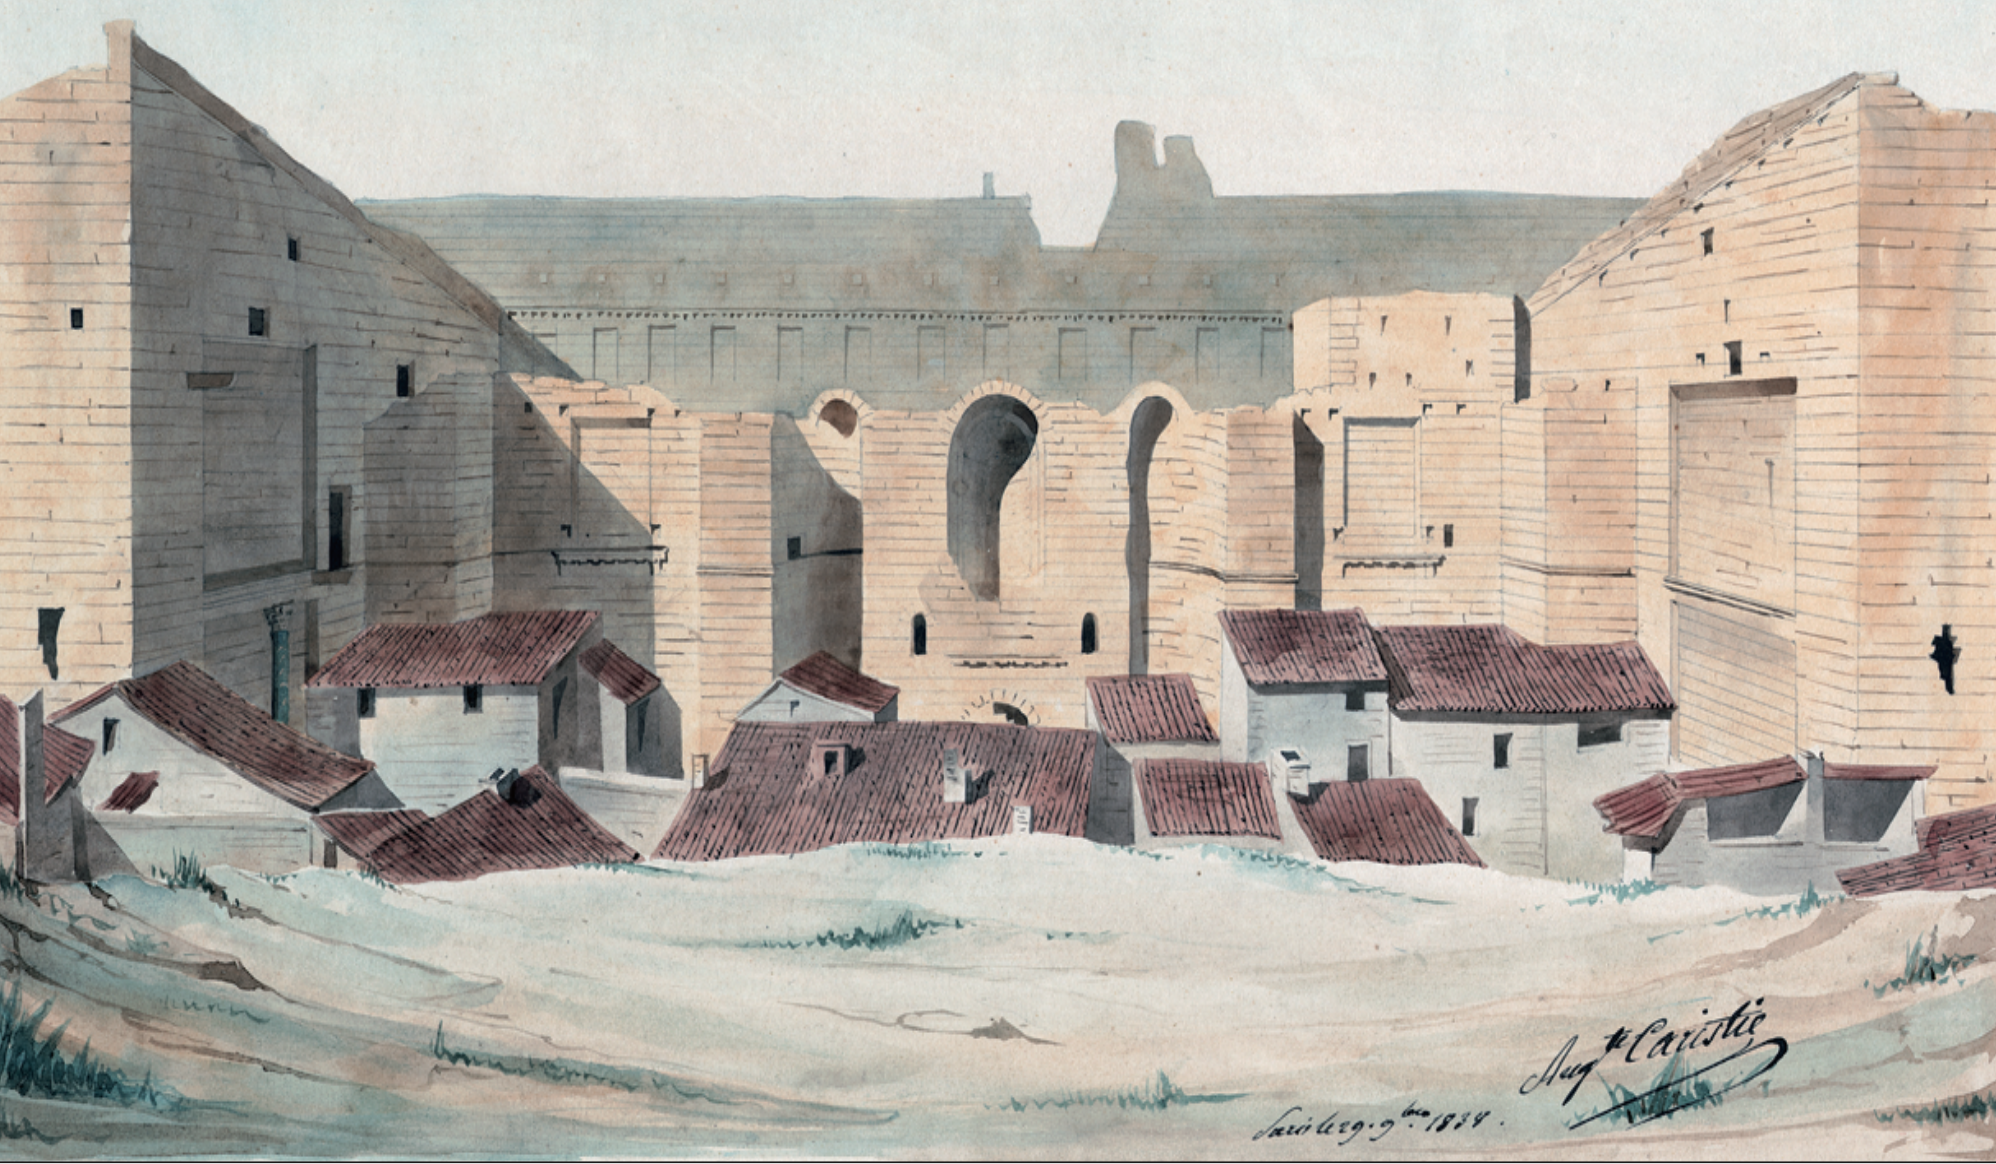
\includegraphics[width=\linewidth]{images/av_deblaiement}
		\caption{Vue de la scène avant le déblaiement par A. Caristie, 1856 (cliché Médiathèque de l’Architecture et du Patrimoine, Charenton)}
	\end{subfigureth}
	\begin{subfigureth}{0.47\textwidth}
		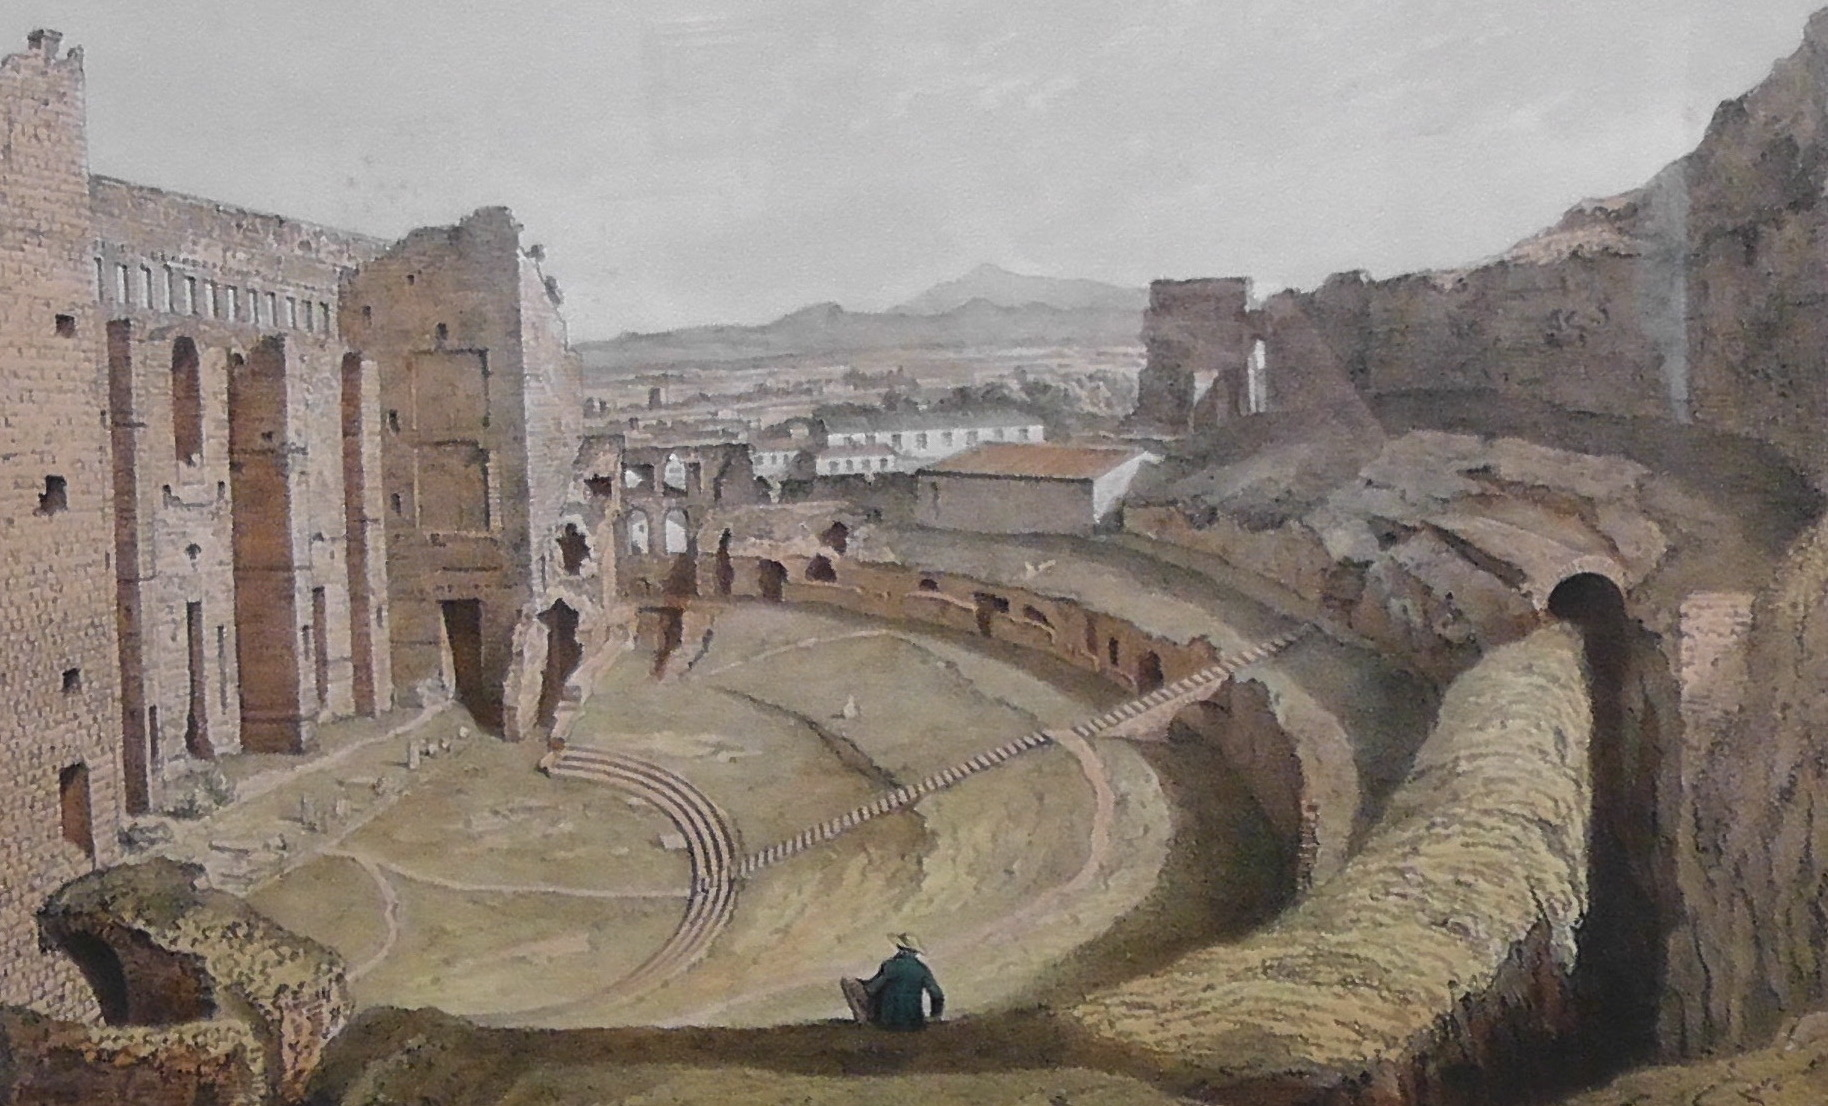
\includegraphics[width=\linewidth]{images/asselineau}
		\caption{Vue intérieure du théâtre, par Asselineau, XIX\up{e} siècle, Musée d'Art et d'Histoire d'Orange}
	\end{subfigureth}
	\caption[Théâtre d'Orange avant restauration]{Dessins du théâtre d'Orange avant et après déblaiement par A.Caristie}		
	%\label{fig:caristie}
\end{figureth}		

		
	\chapter{Architecture générale du théâtre d'Orange}
		\citationChap{
		L'architecture, c'est ce qui fait les belles ruines
		}{Auguste Perret}
		\minitoc
		\newpage
		
		\section{Introduction}
		
		En 2013, l'\gls{iraa} lance une série de campagnes de mesure et d'analyse du théâtre d'Orange d'une part grâce à des relevés effectués sur le terrain et d'autre part à l'aide d'une étude approfondie des documents d'archive conservée pour la plupart à la Médiathèque de l'architecture et du patrimoine à Charenton-le-Pont. Celles-ci comportent les plans de Caristie et Daumet et permettent d'avoir une vision du théâtre avant que celui-ci ne soit restauré par Formigé. L'étude réalisé durant cette thèse est donc principalement basée sur le rapport de l'\gls{iraa} résultant de ces travaux d'analyse : \cite{orangeTxt} et \citep{orangePl}.
		
		Le théâtre d'Orange a été bâtie en partie selon les indications de \cite{vitruve} et suit donc les préceptes de l'architecture romaine de l'époque impériale. Comme la plupart de ces édifices, il se présente en demi-cercle fermé par un mur rectiligne. Sa \gls{cavea} tournée vers le Nord est adossée à la colline Saint-Eutrope offrant ainsi un support naturel à l'édifice. A la différence des \glspl{odeon} seul un \gls{velum} servait de toiture aux spectateurs.

\begin{figureth}
		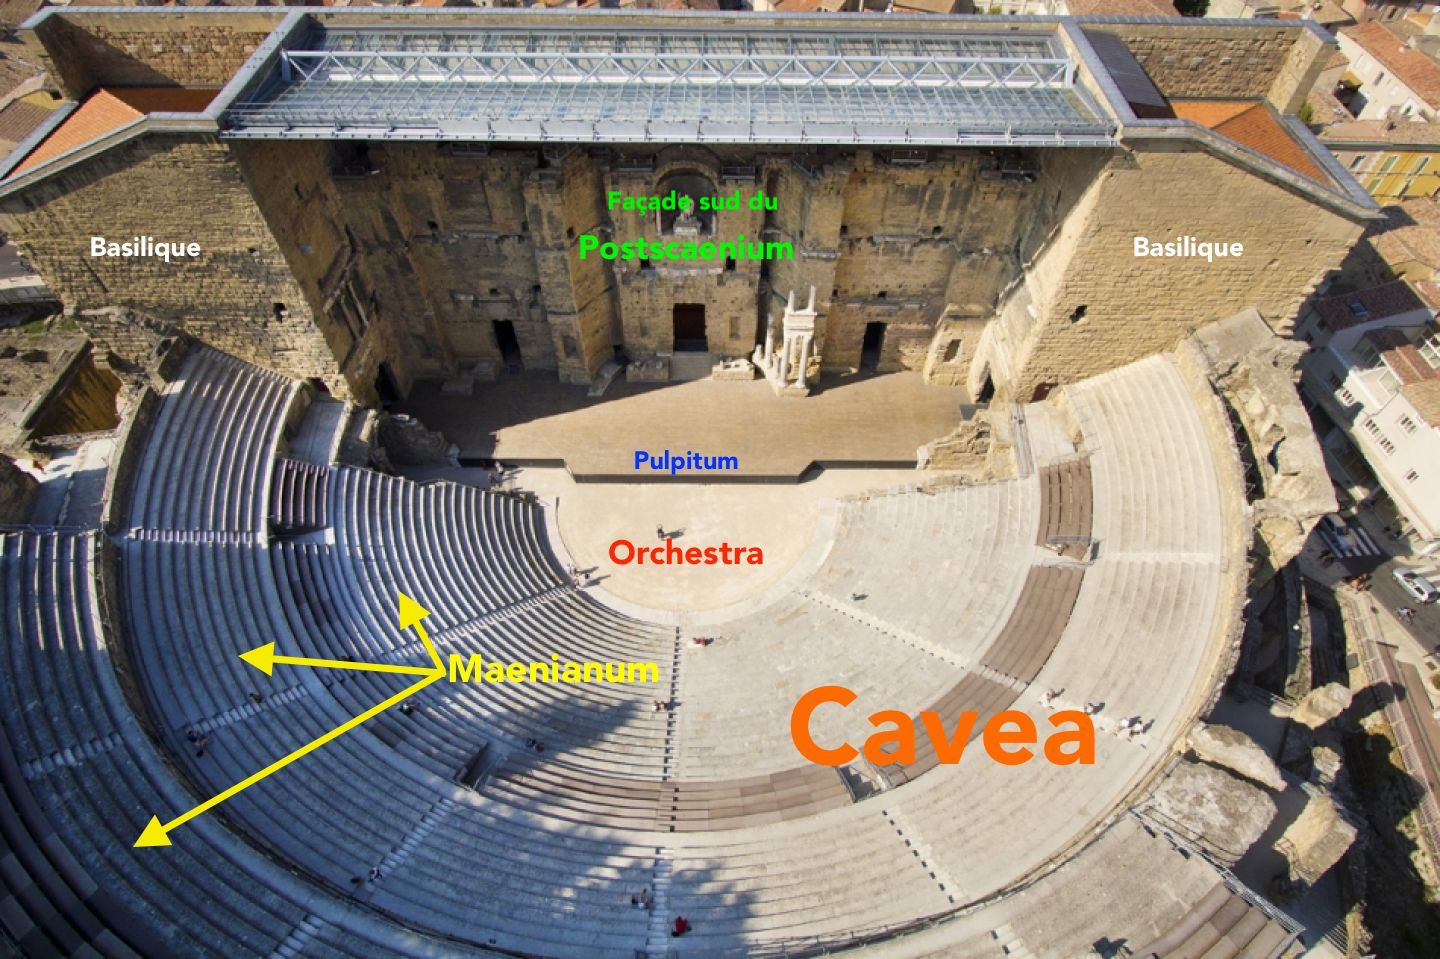
\includegraphics[width=\linewidth]{images/vuensemble}
		\caption[Vue d'ensemble du théâtre d'Orange]{Vue d'ensemble du théâtre d'Orange (cliché de Boudereaux sur choregies.fr)}
\end{figureth}


		\section{Le \gls{postscaenium} et les \glspl{basilique} }
		
		Le \gls{postscaenium} (ou mur de scène) constituant la façade nord du bâtiment ainsi que les deux \glspl{basilique} l'enclavant constituent les parties les mieux conservées du théâtre. Le \gls{postscaenium} servait de décor pour les représentations et tenait probablement un rôle acoustique (voir \Nameref{part3}). Les côtés est et ouest donnaient sur des rues, alors qu'adossé à la façade nord se trouvait une \gls{porticus ps} servant de galerie commerçante. Celui-ci se trouvant à l'extérieur du théâtre, il ne fera pas partie de l'étude. Il donne néanmoins accès au \gls{postscaenium} par le biais de dix-sept portes reparties de manière symétrique par rapport à la porte centrale. Sur la partie haute de la façade se trouve deux séries de \glspl{console} ainsi qu'une assise de bouches d'eau qui permettaient d'évacuer les eaux qui tombaient sur le toit du bâtiment de scène. Les \glspl{console} de la série supérieure (mis à part les deux situées aux extrémités) présentent un trou traversant permettant d'accueillir le mât. Celles de la série inférieure sont creusées à leur lit d'attente
d'une grande mortaise circulaire prolongée par un petit trou permettant l'écoulement de l'eau de pluie. Pour pouvoir placer un mât dans un couple \glspl{console} il fallait également que l'assise de bouche d'eau soit percée. Or cela n'est le cas que pour douze emplacements correspondant aux mâts n\no4 à 9 à partir des deux extrémités du mur. Il semble que les mâts n'aient été présents qu'à ces emplacements, c'est à dire au niveau des \glspl{basilique} et non du mur de scène pour soulager ce dernier d'une trop forte tension liée au poids du \gls{velum}. L'intérieur du \gls{postscaenium} comporte huit pièces donnant uniquement sur la \gls{porticus ps} à l'extérieur du théâtre. Trois portes dont la porte royale donnent directement accès à la scène. Deux portes de part et d'autre amène aux \glspl{basilique} et une au \gls{parascaenium} et à des escaliers permettant de monter aux étages supérieurs. \`{A} l'intérieur du \gls{postscaenium}, en plus du rez-de-chaussé et des combles, on compte deux étages assurés par la présence de baies à arcature permettant de passer d'une pièce à l'autre à l'intérieur du mur. Cela permettait aux acteurs d'accéder à des niches traversante en hauteur pour faire apparaitre par exemple des personnages divins ou effectuer des bruits de tonnerre. 
		
		La façade sud du mur (ou front de scène) est celle qui servait de décor aux spectacles. Aujourd'hui, il ne reste que le mur en calcaire de Courthézon (calcaire de couleur jaune foncé-beige) qui été jadis caché par des ornementations en marbre. On y trouve plusieurs niches de diverse profondeurs ainsi que les traces d'encastrement du placage de marbre qui servent de repère aux archéologues pour reconstituer la décoration. Le mur a une géométrie symétrique par rapport à l'axe décrit par la porte royale rectangulaire et la niche voutée située au dessus et accueillant aujourd'hui une statue dite "d'Auguste" (faite de ciment et de fragments antiques et placée là en guise de décoration en 1944). Cet axe est placé sur une paroi rectiligne qui fait saillie au fond d'une \gls{exedre} curviligne ce qui donne un effet de "focus" vers la porte royale et la niche voutée. De part et d'autre se trouvent deux  \glspl{exedre} rectangulaires peu profondes. Le mur est découpé verticalement en trois ordres sur les extrémités et seulement deux sur la partie centrale. Au dessus se trouve l'espace réservé au toit qui couvrait le \gls{postscaenium} et la scène. On y voit aujourd'hui les trous d'encastrement dans lesquelles venaient s'insérer les poutres.
		
		Le mur de façade du bâtiment de scène est flanqué de part et d'autres de deux \glspl{basilique} de forme presque carrée auxquelles on accède depuis la scène par une grande porte rectangulaire et un \gls{parascaenium}. Les \glspl{basilique} servaient à entreposer des décors volumineux et permettaient l'entrée des artistes. Elles donnaient également accès à l'extérieur ou aux \gls{aditus} par un couple de baies à arcature.
		
				
		\section{L'\gls{orchestra}, les \gls{aditus} et la \gls{cavea}}
		
	
	L'\gls{orchestra} est la partie semi-circulaire situé entre la scène et le premier gradin. Anciennement nommée "choros", chez les grecs qu'elle y accueillait le choeur, elle ne sert plus aux représentations chez les romains et certains spectateur de marque pouvaient s'y installer. Aujourd'hui recouverte de graviers compact elle pouvait être à l'époque dallée de marbre ou pavé de pierres colorées. L'\gls{orchestra} était limité par un \gls{balteus} qui marquait la séparation avec la \gls{cavea} et qui surplombait un petit caniveau permettant d'évacuer l'eau de pluie.
	
Depuis l'extérieur du théâtre on accède à ce lieu par deux larges \gls{parodos} formant les \gls{aditus}. Chacune est composée d'une succession de trois voûtes en décrochement qui portaient les tribunes et les extrémités de la  \gls{cavea}.
	
		La  \gls{cavea}, telle qu'elle a été restaurée, comprend trois hémicycles appelés \gls{maenianum}, séparée l'un de l'autre par une \gls{precinction} et un \gls{podium}. Cela a été déduit par Caristie de par la forme des \gls{aditus}, les vestiges du premier gradin et de la première \gls{precinction} et reconstruit en ce sens par Formigé. Chaque \gls{maenianum} est divisé en un certains nombre de sections appelées \gls{cuneus} par des escaliers.
Le premier \gls{maenianum}, ou \textit{ima cavea} séparé en quatre \gls{cuneus}, comprend un repose-pied à sa base et vingt gradins. Au niveau de la première \gls{precinction} neuf ouvertures donnent  sur un couloir souterrain (premier \gls{ambulacre}). Ce dernier est accessible depuis l'extérieur du théâtre au rez-de-chaussée par deux escaliers longeant les \gls{aditus}. Le couloir ouvre aussi sur dix-huit pièces aveugles, mais seule les salles numérotées de 1 à 8 (\ref{1erniveau}) sont des constructions antiques. Il était également possible de rejoindre le premier \gls{maenianum} à mi-hauteur depuis les \gls{parodos} par le biais de deux escaliers installés sous les gradins. Ceux-ci n'ont pas été remis en fonction lors de la restauration.
		
	\begin{figureth}
		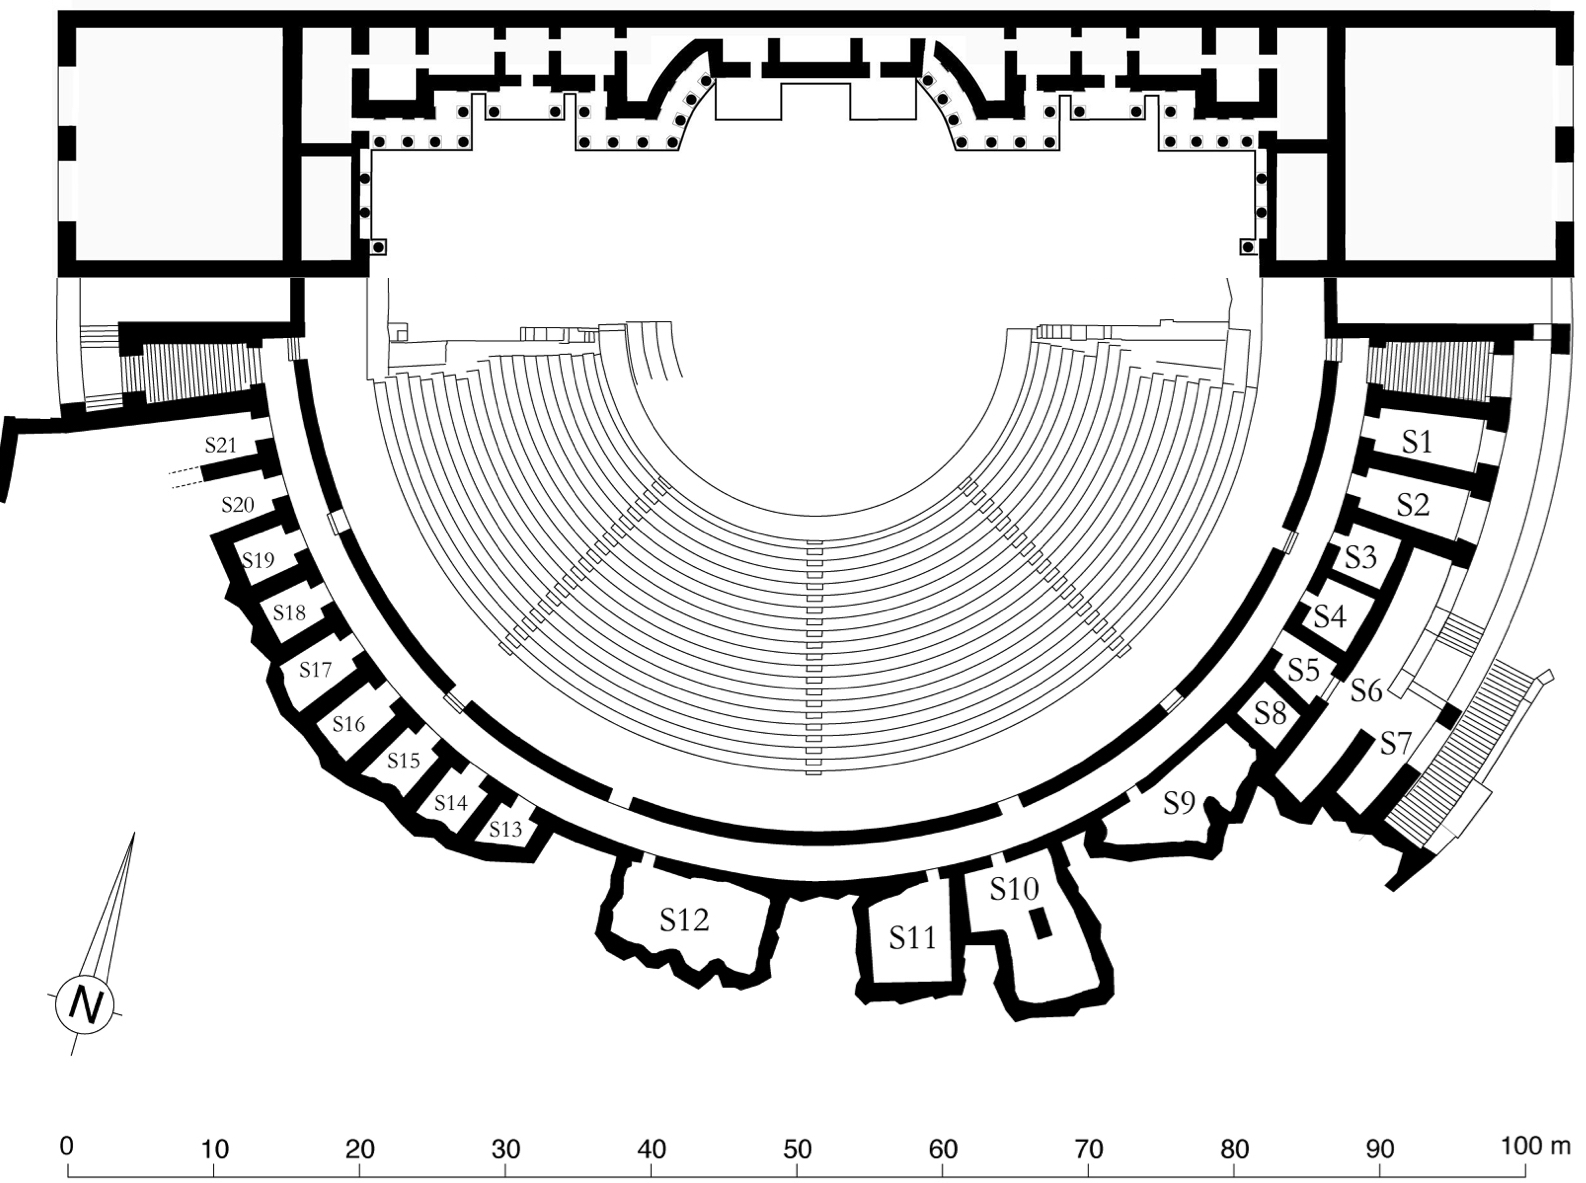
\includegraphics[width=\linewidth]{images/1erniveau}
		\caption[Vue de dessus - 1er niveau]{Plan du théâtre au niveau du premier ambulacre \cite[Pl. XVII]{orangePl}}
		\label{1erniveau}
	\end{figureth}		
		
Le deuxième \gls{maenianum}, ou \textit{media cavea}, repose, dans sa partie inférieure, sur l'\gls{ambulacre} du premier niveau et, dans sa partie supérieure, sur de la terre ou du remblai que complète, à proximité des aditus, deux niveaux de chambres voûtées. 
		
		
		Il comporte, entre deux circulations horizontales peu profondes, neuf gradins
divisés en huit cuneus par neuf escaliers. On accède à son niveau supérieur par une série de
passages radiaux reliés à un second couloir annulaire, dont la paroi extérieure s'identifie au
mur périphérique du théâtre. Cinq de ces passages, qui devaient être neuf dans l'Antiquité,
sont aujourd'hui utilisables. Le couloir est souterrain dans la zone où la cavea est adossée et
construit sur deux niveaux de chambres voûtées dans sa partie la plus orientale. Il est
directement accessible de l'extérieur par une porte à l'est et une autre à l'ouest.
		
	\begin{figureth}
		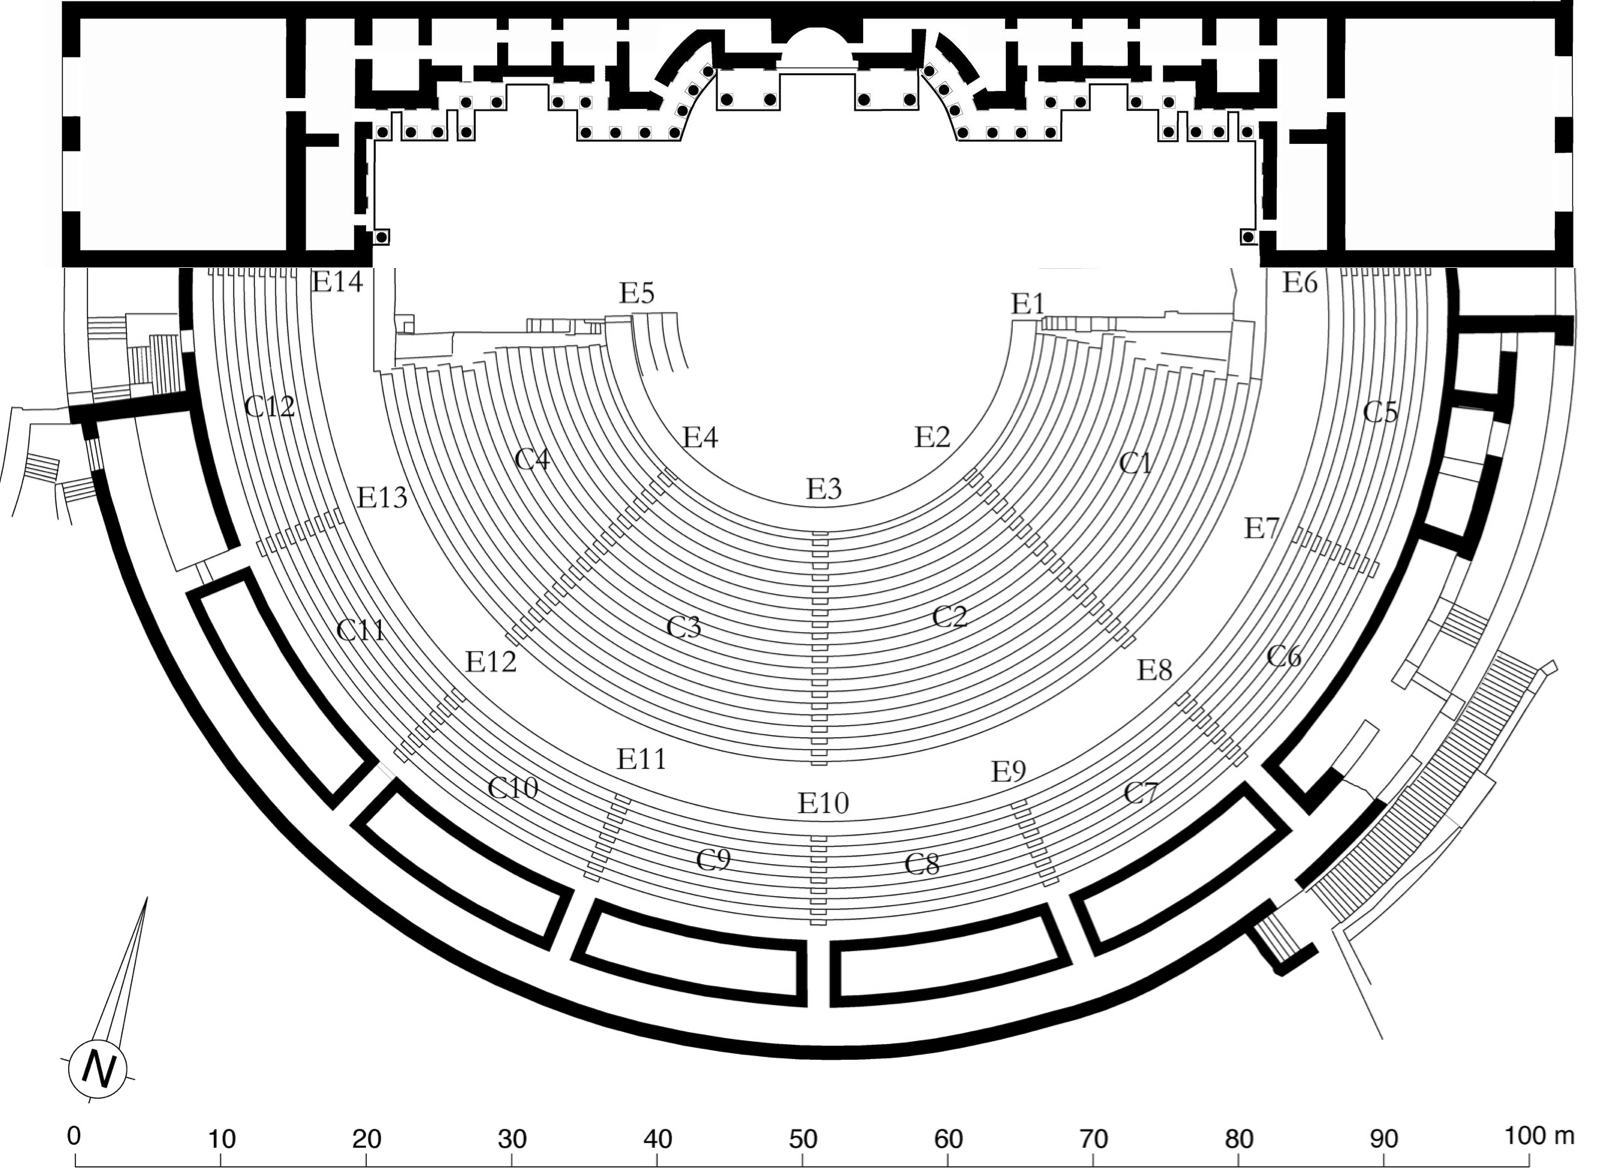
\includegraphics[width=\linewidth]{images/2emeniveau}
		\caption[Vue de dessus - 2ème niveau]{Plan du théâtre au niveau du second ambulacre \cite[Pl. XVIII]{orangePl}}
		\label{2emeniveau}
	\end{figureth}		
		
		
Le troisième maenianum, ou summa cavea, est entièrement construit sur structure creuse. Il comporte cinq gradins à l'origine divisés par neuf escaliers. Il est couronné par une
plate-forme aménagée au-dessus du second couloir annulaire. Celle-ci était jadis occupée
par un portique, une porticus in summa cavea, dont la reconstruction partielle de deux
colonnes évoque la présence. Dans sa partie centrale, le mur périphérique de la cavea est
percé de portes donnant accès au portique et à la summa cavea à partir du chemin qui borde
l'édifice à sa périphérie. Les portes sont axées sur les escaliers de la cavea.

	\begin{figureth}
		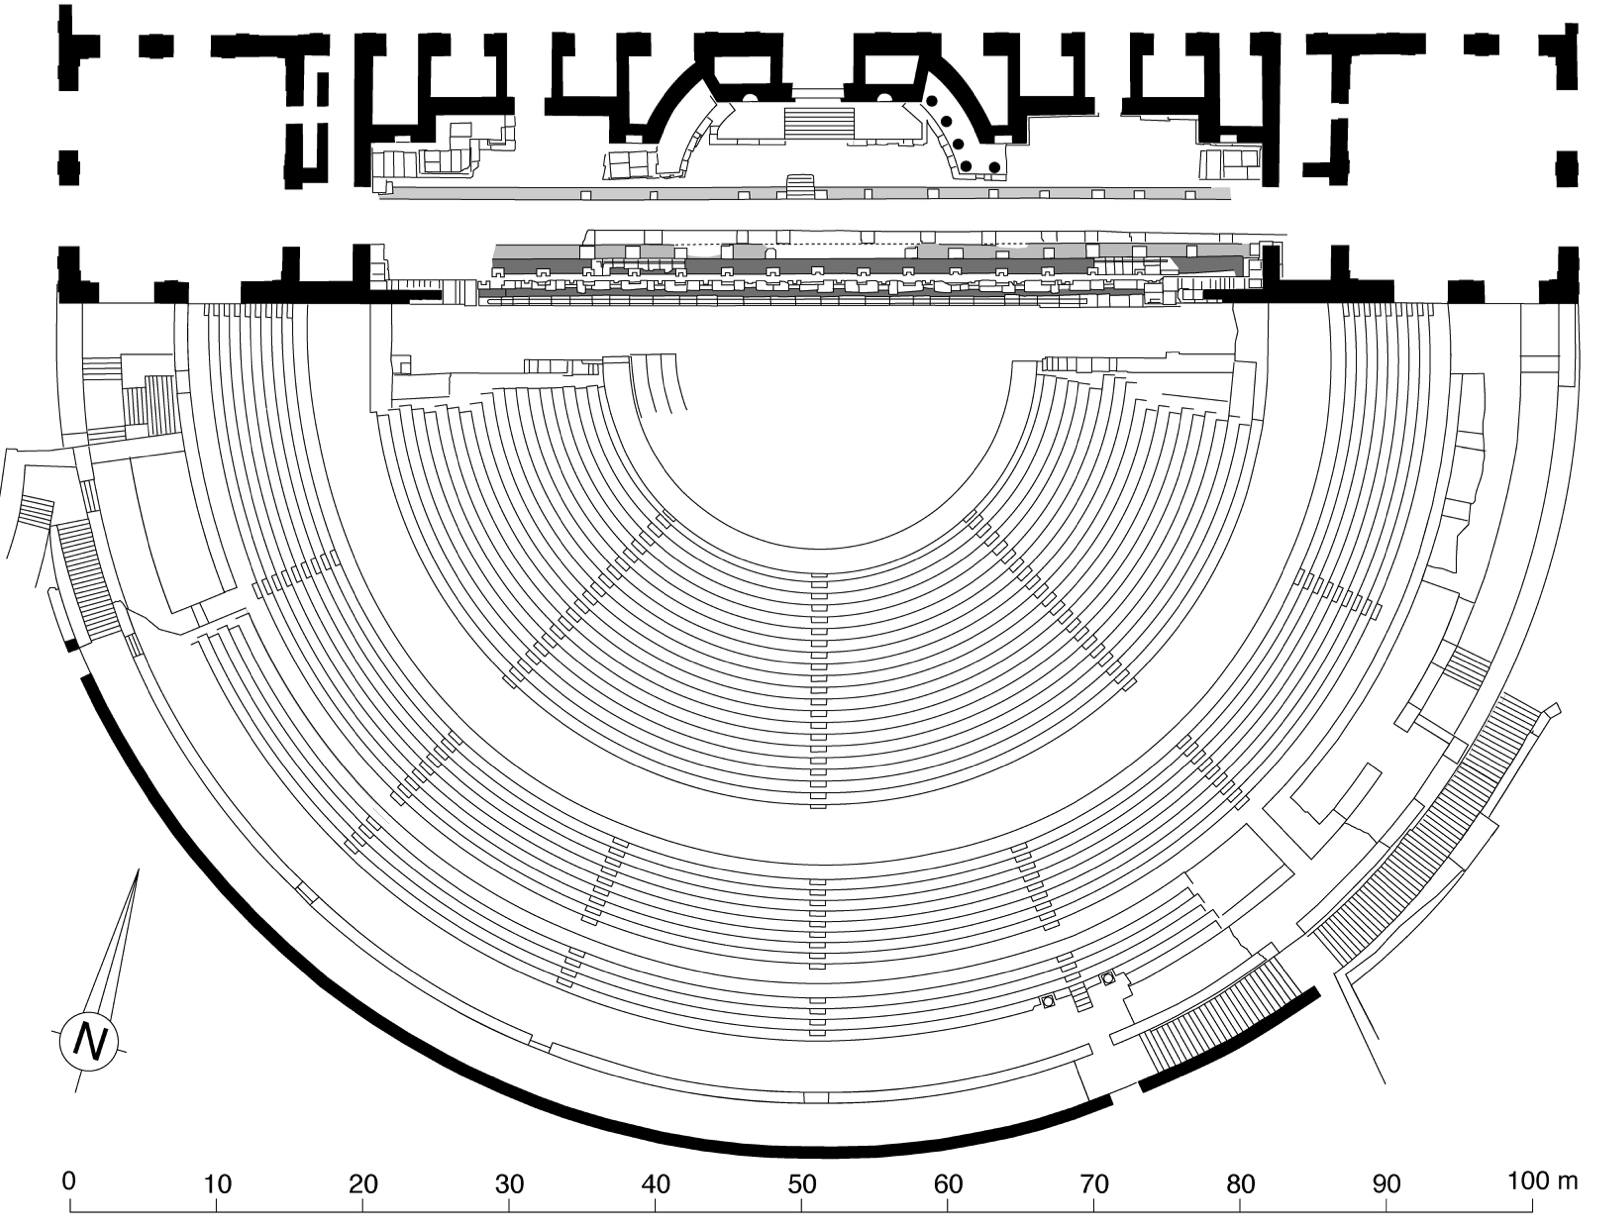
\includegraphics[width=\linewidth]{images/3emeniveau}
		\caption[Vue de dessus - 3ème niveau]{Plan du théâtre au niveau de la rue périphérique \cite[Pl. XIX]{orangePl}}
		\label{2emeniveau}
	\end{figureth}	
		
		
		\section{Les couvertures et le velum}
		
\begin{figureth}
		%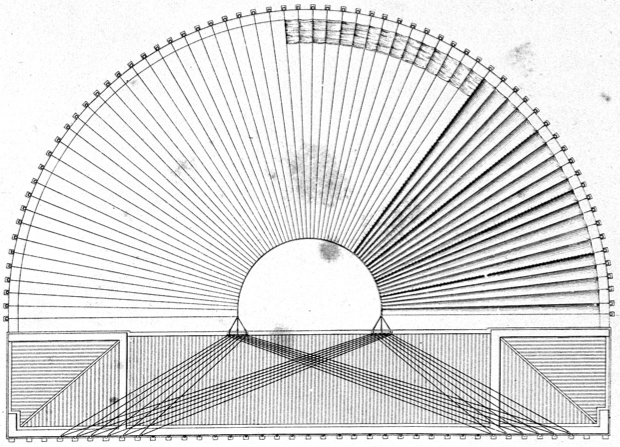
\includegraphics[width=\linewidth]{images/velumCaristie}
		\caption[Velum]{proposition de restitution du velum d'Orange par A.Caristie}
		
\end{figureth}		

		\section{Exemple minimal}
		
			\subsection{Exemple Tableaux et figures}
			On va ici placer des éléments graphiques (voir tableau~\ref{tab:exemple} et figure~\ref{fig:exemple}), juste pour avoir des entrées dans les listes des figures et des 	tableaux. On remarquera l'utilisation des sous-figures~\ref{sub:Antibes} et~\ref{sub:SaintJeannet}.
	
			\begin{tableth}
				\caption[Légende courte pour l'exemple de tableau]{Un tableau avec une légende tellement longue que ce serait hideux dans la liste des tableaux}
					\label{tab:exemple}
				\begin{tabular}{c|c}
					Coucou	& Au revoir\\
					\hline
					maman	& papa
				\end{tabular}
			\end{tableth}
	
			\subsection{Exemple Symboles mathématiques}
			Rien de spécial à propos des math, hormis l'illustration des symboles listés en fin de document, tels \gls{alpha} ou \gls{gamma}, qui peuvent être utilisés indifféremment en mode \emph{in-line} ou dans des équations\footnote{Le lecteur notera que \texttt{hyperref} ajoute un lien cliquable sur chaque entrée des différents glossaires.} :
			\begin{equation}
				\gls{alpha}=\nicefrac{\gls{gamma}}{2}
				\label{eq:alphagamma}
			\end{equation}
			Les entrées des glossaires peuvent même être appelés dans des figures (PDF avec surcouche \LaTeX, ou Ti\textit{k}Z).
	




	\chapter{Modélisation}
		\citationChap{
			Les détails font la perfection et la perfection n'est pas un détail
		}{Léonard de Vinci}
		\minitoc
		\newpage
		
		\section{Introduction}
		Pour pouvoir étudier un monument dans ces moindres détails de nombreux chercheurs s'orientent aujourd'hui vers la modélisation 3D. Effectivement, jusqu'à présent les scientifiques menaient leurs études à l'aide de plans ou de dessins en 2D ou bien de maquette à échelle réduite. Mais les outils numériques disponibles aujourd'hui comportent de nombreux avantages par rapport à ces anciennes techniques. Tout d'abord, il est possible d'obtenir les mêmes informations qu'avec les "anciennes techniques" en terme de côtes, formes, aspect. Mais en plus, à partir d'un modèle numérique unique, on peut sélectionner les informations que l'on souhaite étudier tout simplement en changeant les objets à afficher, les vues ou les modes d'affichage. On peut par exemple afficher un monument par vu du dessus avec ses cotes et étudier le plan 2D correspondant. Mais on peut également réaliser une impression 3D pour en avoir une maquette à l'échelle réduite. Un seul outil permet donc d'obtenir l'ensemble des informations que l'on souhaitait acquérir par le passé. Un modèle numérique 3D peut par ailleurs être utilisé par des logiciels de calcul ou de simulation afin de tester des hypothèses physiques (écoulement de fluide, acoustique, ...) ou architecturale (portance, agencement de décor, ...). Il permet également de réaliser des animations (déplacement de personnages, ouverture de haut-vents, ...) ou des visites immersives grâce aux technologies de réalité virtuelle. 

Il existe bien entendu de nombreuses limites à la numérisation 3D car cette technique est relativement récente et beaucoup de développement sont en cours. La principale contrainte est la puissance de calcul des ordinateurs et leur espace de stockage qui doivent prendre en charge de très grandes quantités de données.

Pour virtualiser des monuments, il y a deux techniques principalement utilisées. La première consiste à réaliser un nuage de point à l'aide d'appareils de mesure (laser, appareils photo, ...) à la manière d'un scanner. Prenons l'exemple de la photogrammetrie qui est aujourd'hui largement répandue dans la restitution numérique de monument. Il s'agit de photographier l'ensemble du bâtiment sous tous ses angles en s'assurant que chaque photo a une partie commune avec une autre. Les logiciels de traitement peuvent alors corréler les photos les unes avec les autres et recréer l'image en trois dimensions. Cependant, la limite de cette technique est que plus la précision est grande, plus le volume de donnée à traiter est conséquent et rend les calculs difficiles. C'est pourquoi nous avons utiliser la deuxième méthode dite de CAO (conception assistée par Ordinateur). Il s'agit de retranscrire par des formes géométriques 3D plus ou moins complexes le monuments.


		\section{Le mur de scène et ses basiliques}

Le mur de scène ainsi que ses deux basiliques constituent un bloc distinct. Le contour extérieur est créé grâce aux cotes de la planche XXI \cite{ref2}. Ce bloc est disposé dans le repère absolu d'après les cotes indiquées sur le plan nord-sud par rapport au centre de révolution de la cavea. Sur le plan est-ouest, le mur de scène extérieur (la plus grande longueur) est centré en 0, les extrémités de chacune des basiliques sont donc à 51,96m du centre.

Sont ensuite crées des objets représentant les pièces. A l'aide d'un modifier Boolean ces objets sont soustraits à la forme de base. La même méthode est utilisée pour le haut du mur qui supporte le toit (fig 24 \cite{ref},  pour les ouvertures sur le front de scène (planche XXIX \cite{ref2}), et pour les portes (planche XXI \cite{ref2}). Pour l'encastrement des poutres dans la partie sommitale du mur nous utilisons des poutres rectangulaire et identique car les traces décrites sur la planche XXXVII \cite{ref2} sont difficiles à interprétation. Cet élément pourra être corrigé par les archéologues dans une prochaine étape.

		\section{Le pulpitum et l'orchestra} 

Le pultpitum, autrement dit l'estrade de scène a complètement disparu et a aujourd'hui été remplacé par un plancher moderne. Il reste néanmoins des traces sur le mur de scène qui permettent de le modéliser dans sa version antique. Les planches XLVII et XLIX \cite{ref2} donnent les élévations du pulpitum ainsi que de l'orchestre sure les extrémités orientales et occidentales. L'orchestre est une forme volumique dont la face supérieure représente le sol. Il sera dans une prochaine étape creusé à l'aide de modifiers Boolean pour l'hyposcaenium et le caniveau décrit dans une autre partie.

		\section{La colline Saint-Eutrope} 
Comme souvent les architectes de l'époque ont adossé la cavea sur un relief naturel afin de solidifier la structure et de simplifier la construction de l'édifice. La colline Saint-Eurtope qui soutient donc le théâtre sur sa partie méridionale a été modélisée d'après les lignes d'altitude (référencées page 11 \cite{ref}) à partir de la plus basse jusqu'à la plus haute par pas de 6m par extrusion successive. Les élévation ont ensuite été légèrement adaptée (ligne par ligne) pour s'encastrer au mieux dans le théâtre. La colline est donc actuellement peu précise et il est nécessaire de l'affiner à l'aide d'un document détaillant mieux sa géométrie.

		\section{La cavea} 

La cavea est la partie semi-circulaire adossée à la colline qui soutien les maenianum (gradins). Elle comporte des ambulacres qui permettent aux spectateurs d'atteindre leur siège par le biais de vomitorium et s'ouvre sur les rues extérieures par trois étages d'arcades. La modélisation se fait à partir de la planche LX \cite{ref2} en plaçant la bordure extérieure au même niveau que la bordure des basilique (c'est à dire à 51,96m du centre). Une fois le plan de coupe réalisé on utilise un modifier Screw pour faire une extrusion circulaire autour du centre. On comprend alors que les cotes de l'ensemble de la cavea sont celles de la coupe théorique. Sur cette planche certaines valeurs sont incohérentes et on utilise donc la règle décrite en introduction de cette partie pour choisir les bonne valeurs.
Le troisième maenianum n'étant pas soutenu par la colline, il repose sur des caissons voûtés qui sont modélisés séparément. 

Les arcades donnant sur l'extérieur sont répétées à l'aide d'un modifier Array puis soustraites à la cavea par un modifier Boolean. A noter que le modifier Screw doit être appliqué pour que le Boolean fonctionne.

		\section{Maenianum} 

Les Maenianum sont modélisés à partir d'un plan de coupe d'un bloc formant un gradin auquel est appliqué un modifier Array (dupliquant du nombre de gradins) et d'un modifier Screw pour faire une extrusion de révolution. Le plan de base est un quasi-triangle représentant le profil d'un bloc rectangulaire coupé en deux. Il n'est pas coupé le long de la diagonale car une partie plate d'une dizaine de centimètre permet de faire reposer les bloc les une sur les autres. Cette forme est issue du document \cite{ref} où l'on retrouve "le seul gradin antique dont une face de joint est actuellement visible" figure \ref{coupeGradin}. C'est cette forme qui est ajustée pour coïncider avec les cotes de la cavea. Une fois les modifiers appliqués, on peut utiliser un nouveau modifier Boolean pour les marches d'escalier et les vomitorium. Les empruntes des escaliers qui seront retirés aux maenianum sont en fait la forme de base du maenianum retourné et placé de sorte que le coin supérieur (le bord du gradin) se retrouve au centre de la partie visible du gradin. Cela permet de retirer exactement la moitié de la hauteur et de la profondeur du gradin. La forme 2D de l'escalier est ensuite dupliqué avec le modifier Array et extrudé avec un modifier Solidify sur 1,2m. Cette valeur est prise arbitrairement par rapport aux plans non coté du document \cite{ref2} et devra être affinée par les experts.

		\begin{figure}[!h] %on ouvre l'environnement figure
			\center
			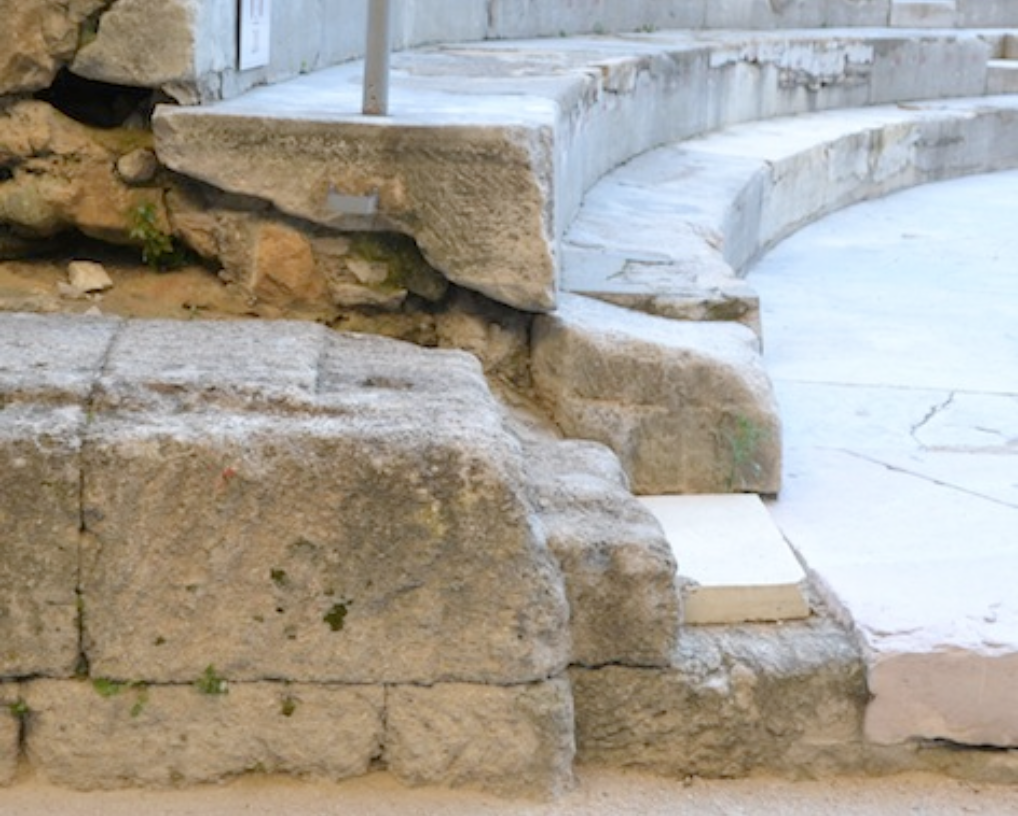
\includegraphics[scale=0.3]{images/gradinCoupe}
			\caption[Repose pied et premier gradin du premier cuneus]{Le repose pied et le premier gradin du premier cuneus : vu de l'extrémité nord avec au premier plan, le mur bordant l'aditus est} %la légende
			\label{coupeGradin} %l'étiquette pour faire référence à cette image	
		\end{figure} %on ferme l'environnement figure 
		
		\begin{figure}[!h] 
			\center
			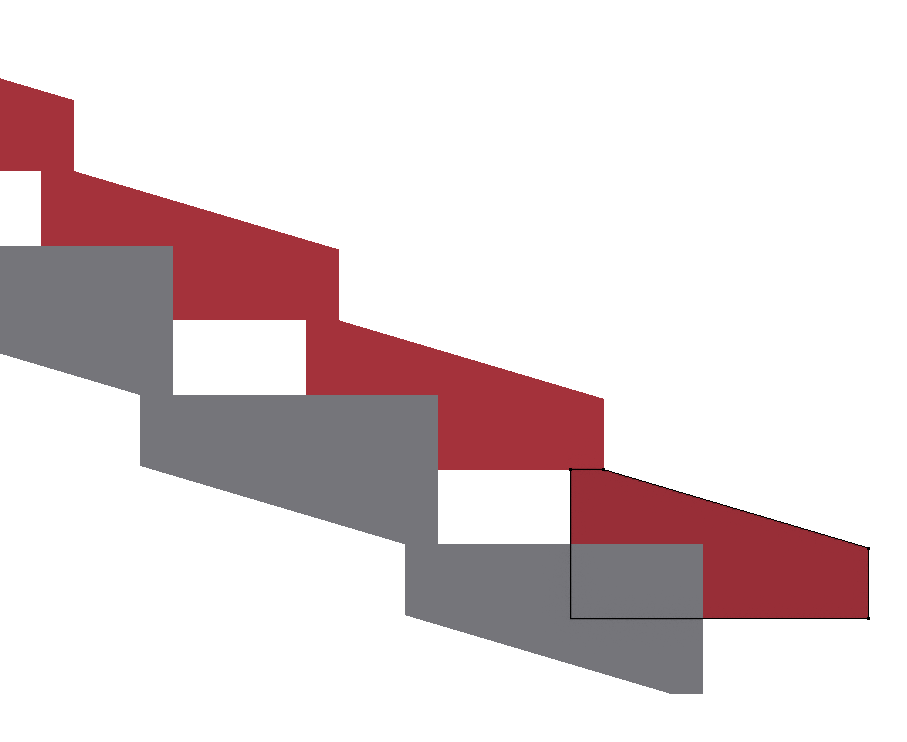
\includegraphics[scale=0.3]{images/escaliers}
			\caption[Modélisation des maenianum]{Modélisation des maenianum et de l'emprunte des escaliers à retirer apres application des modifers Array et Screw}
		\end{figure}
		
		\section{Aditus} 

		
	\chapter{Propositions de reconstitution}
		\citationChap{
		The thing about quotes on the internet is that you can not confirm their validity
		}{Abraham Lincoln}
		\minitoc
		\newpage
		
	\chapter*{Conclusion}
	\addcontentsline{toc}{chapter}{Conclusion}
		\newpage
			
% Biblio
%\titleformat{\chapter}[hang]{\bf\huge}{}{2pc}{} % Pour enlever "Chapitre N"
 %\titleformat{\chapter}[display]{\bf\huge}{Chapitre \thechapter}{2pc}{} % Pour remettre "Chapitre N"
 \bibliographystyle{francaissc}
 \bibliography{Part1/Biblio}
\addcontentsline{toc}{chapter}{Références}


